\documentclass[14pt]{extbook}
\usepackage{multicol, enumerate, enumitem, hyperref, color, soul, setspace, parskip, fancyhdr} %General Packages
\usepackage{amssymb, amsthm, amsmath, bbm, latexsym, units, mathtools} %Math Packages
\everymath{\displaystyle} %All math in Display Style
% Packages with additional options
\usepackage[headsep=0.5cm,headheight=12pt, left=1 in,right= 1 in,top= 1 in,bottom= 1 in]{geometry}
\usepackage[usenames,dvipsnames]{xcolor}
\usepackage{dashrule}  % Package to use the command below to create lines between items
\newcommand{\litem}[1]{\item#1\hspace*{-1cm}\rule{\textwidth}{0.4pt}}
\pagestyle{fancy}
\lhead{Progress Quiz 10}
\chead{}
\rhead{Version A}
\lfoot{6232-9639}
\cfoot{}
\rfoot{Fall 2020}
\begin{document}

\begin{enumerate}
\litem{
Determine the appropriate model for the graph of points below.
\begin{center}
    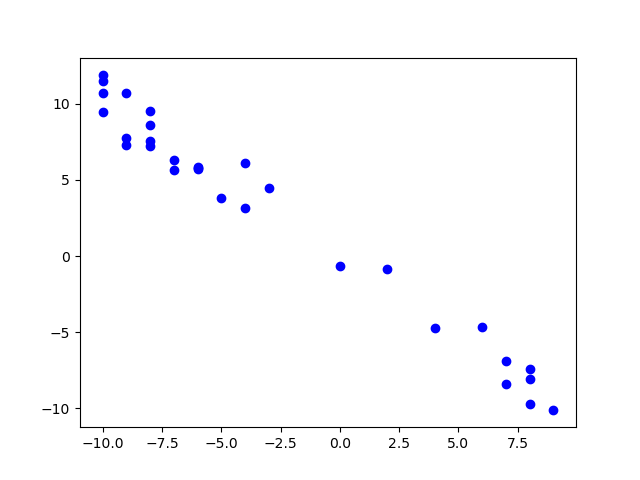
\includegraphics[width=0.5\textwidth]{../Figures/identifyModelGraph12A.png}
\end{center}
\begin{enumerate}[label=\Alph*.]
\item \( \text{Linear model} \)
\item \( \text{Exponential model} \)
\item \( \text{Logarithmic model} \)
\item \( \text{Non-linear Power model} \)
\item \( \text{None of the above} \)

\end{enumerate} }
\litem{
Solve the modeling problem below, if possible.
\begin{center}
    \textit{ In CHM2045L, Brittany created a 15 liter 19 percent solution of chemical $\chi$ using two different solution percentages of chemical $\chi$. When she went to write her lab report, she realized she forgot to write the amount of each solution she used! If she remembers she used 16 percent and 26 percent solutions, what was the amount she used of the 26 percent solution? }
\end{center}
\begin{enumerate}[label=\Alph*.]
\item \( 7.50 \)
\item \( 10.50 \)
\item \( 5.54 \)
\item \( 4.50 \)
\item \( \text{There is not enough information to solve the problem.} \)

\end{enumerate} }
\litem{
Determine the appropriate model for the graph of points below.
\begin{center}
    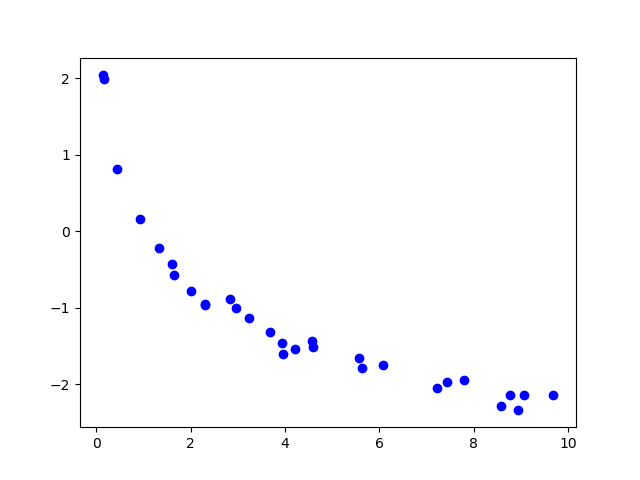
\includegraphics[width=0.5\textwidth]{../Figures/identifyModelGraph12CopyA.png}
\end{center}
\begin{enumerate}[label=\Alph*.]
\item \( \text{Exponential model} \)
\item \( \text{Non-linear Power model} \)
\item \( \text{Linear model} \)
\item \( \text{Logarithmic model} \)
\item \( \text{None of the above} \)

\end{enumerate} }
\litem{
Solve the modeling problem below, if possible.
\begin{center}
    \textit{ A new virus is spreading throughout the world. There were initially 7 many cases reported, but the number of confirmed cases has doubled every 5 days. How long will it be until there are at least 100000 confirmed cases? }
\end{center}
\begin{enumerate}[label=\Alph*.]
\item \( \text{About } 22 \text{ days} \)
\item \( \text{About } 48 \text{ days} \)
\item \( \text{About } 70 \text{ days} \)
\item \( \text{About } 20 \text{ days} \)
\item \( \text{There is not enough information to solve the problem.} \)

\end{enumerate} }
\litem{
For the scenario below, use the model for the volume of a cylinder as $V = \pi r^2 h$.
\begin{center}
    \textit{ Pringles wants to add 36 \text{percent} more chips to their cylinder cans and minimize the design change of their cans. They've decided that the best way to minimize the design change is to increase the radius and height by the same percentage. What should this increase be? }
\end{center}
\begin{enumerate}[label=\Alph*.]
\item \( \text{About } 3 \text{ percent} \)
\item \( \text{About } 17 \text{ percent} \)
\item \( \text{About } 18 \text{ percent} \)
\item \( \text{About } 11 \text{ percent} \)
\item \( \text{None of the above} \)

\end{enumerate} }
\litem{
For the scenario below, model the rate of vibration (cm/s) of the string in terms of the length of the string. Then determine the variation constant $k$ of the model (if possible). The constant should be in terms of cm and s.
\begin{center}
    \textit{ The rate of vibration of a string under constant tension varies based on the type of string and the length of the string. The rate of vibration of string $\omega$ decreases as the square length of the string increases. For example, when string $\omega$ is 4 mm long, the rate of vibration is 20 cm/s. }
\end{center}
\begin{enumerate}[label=\Alph*.]
\item \( k = 125.00 \)
\item \( k = 320.00 \)
\item \( k = 1.25 \)
\item \( k = 3.20 \)
\item \( \text{None of the above.} \)

\end{enumerate} }
\litem{
Solve the modeling problem below, if possible.
\begin{center}
    \textit{ In CHM2045L, Brittany created a 16 liter 7 percent solution of chemical $\chi$ using two different solution percentages of chemical $\chi$. When she went to write her lab report, she realized she forgot to write the amount of each solution she used! If she remembers she used 5 percent and 19 percent solutions, what was the amount she used of the 5 percent solution? }
\end{center}
\begin{enumerate}[label=\Alph*.]
\item \( 2.29 \)
\item \( 8.00 \)
\item \( 13.71 \)
\item \( 10.13 \)
\item \( \text{There is not enough information to solve the problem.} \)

\end{enumerate} }
\litem{
Solve the modeling problem below, if possible.
\begin{center}
    \textit{ A new virus is spreading throughout the world. There were initially 6 many cases reported, but the number of confirmed cases has quadrupled every 4 days. How long will it be until there are at least 1000000 confirmed cases? }
\end{center}
\begin{enumerate}[label=\Alph*.]
\item \( \text{About } 20 \text{ days} \)
\item \( \text{About } 18 \text{ days} \)
\item \( \text{About } 49 \text{ days} \)
\item \( \text{About } 35 \text{ days} \)
\item \( \text{There is not enough information to solve the problem.} \)

\end{enumerate} }
\litem{
The temperature of an object, $T$, in a different surrounding temperature $T_s$ will behave according to the formula $T(t) = Ae^{kt} + T_s$, where $t$ is minutes, $A$ is a constant, and k is a constant. Use this formula and the situation below to construct a model that describes the uranium's temperature, $T$, based on the amount of time t (in minutes) that have passed. Choose the correct constant $k$ from the options below.
\begin{center}
    \textit{ Uranium is taken out of the reactor with a temperature of $100^{\circ}$ C and is placed into a $19^{\circ}$ C bath to cool. After 38 minutes, the uranium has cooled to $60^{\circ}$ C. }
\end{center}
\begin{enumerate}[label=\Alph*.]
\item \( k = -0.02346 \)
\item \( k = -0.01743 \)
\item \( k = -0.01812 \)
\item \( k = -0.01792 \)
\item \( \text{None of the above} \)

\end{enumerate} }
\litem{
For the scenario below, use the model for the volume of a cylinder as $V = \pi r^2 h$.
\begin{center}
    \textit{ Pringles wants to add 39 \text{percent} more chips to their cylinder cans and minimize the design change of their cans. They've decided that the best way to minimize the design change is to increase the radius and height by the same percentage. What should this increase be? }
\end{center}
\begin{enumerate}[label=\Alph*.]
\item \( \text{About } 18 \text{ percent} \)
\item \( \text{About } 12 \text{ percent} \)
\item \( \text{About } 20 \text{ percent} \)
\item \( \text{About } 3 \text{ percent} \)
\item \( \text{None of the above} \)

\end{enumerate} }
\end{enumerate}

\end{document}